\documentclass[11pt,a4paper]{article}
\usepackage[utf8]{inputenc}
\usepackage[T1]{fontenc}
\usepackage{tgpagella}
\usepackage[spanish]{babel}
\usepackage{geometry}
\usepackage{booktabs}
\usepackage{xcolor}
\usepackage{titlesec}
\usepackage{fancyhdr}
\usepackage[parfill]{parskip}
\usepackage[expansion=false]{microtype}
\usepackage{hyperref}
\usepackage{setspace}
\usepackage{graphicx}
\usepackage{needspace}
\widowpenalty=10000
\clubpenalty=10000
\displaywidowpenalty=10000

\geometry{top=3.0cm,bottom=3.0cm,left=3.5cm,right=3.5cm}
\setlength{\parskip}{0.65em}
\setlength{\parindent}{0em}

\definecolor{azulai}{RGB}{30,80,140}
\definecolor{doradoai}{RGB}{140,90,0}
\definecolor{grisai}{RGB}{70,70,70}

\titleformat{\section}{\Large\bfseries\color{azulai}}{}{0em}{}[{\color{azulai}\titlerule[0.5pt]}]
\titlespacing*{\section}{0pt}{1.4em}{0.5em}

\titleformat{\subsection}{\large\bfseries\color{doradoai}}{}{0em}{}
\titlespacing*{\subsection}{0pt}{1.0em}{0.35em}

\titleformat{\subsubsection}{\normalsize\bfseries\color{grisai}}{}{0em}{}
\titlespacing*{\subsubsection}{0pt}{0.7em}{0.25em}

\pagestyle{fancy}\fancyhf{}
\rhead{\textcolor{grisai}{\small Maite Barraga — Arquitectura Interna}}
\lhead{\textcolor{grisai}{\small Urano · Neptuno · Plutón}}
\cfoot{\textcolor{grisai}{\small\thepage}}
\renewcommand{\headrulewidth}{0.3pt}

\hypersetup{colorlinks=true,linkcolor=azulai,urlcolor=azulai}
\setstretch{1.25}
\tolerance=1500
\emergencystretch=4em

\begin{document}

% ── Portada ──────────────────────────────────────────────────────────────────
\begin{titlepage}
  \centering
  \vspace*{1.5cm}
  {\Huge\bfseries\color{azulai} Urano · Neptuno · Plutón}\\[0.5cm]
  {\large\color{grisai} Arquitectura Interna}\\[0.3cm]
  {\small\itshape\color{grisai} Procesos profundos de cambio, sensibilidad y transformación}\\[2cm]
  {\huge\color{doradoai} Maite Barraga}\\[1.5cm]
  {\Large 07/01/1971 \quad 12:15}\\[0.3cm]
  {\Large Pamplona, España}\\[0.3cm]
  {\normalsize Lat: 42.8157° \quad Lon: -1.6522° \quad UTC+01:00}\\[0.3cm]
  {\normalsize Ascendente: Aries 6°18' \quad
    MC: Capricornio 3°11'}\\[2cm]
  \begin{tabular}{ll}
    \textbf{Urano:}   & Libra — Casa 7 13°31'  \\
    \textbf{Neptuno:} & Sagitario — Casa 8 2°11' \\
    \textbf{Plutón:}  & Virgo — Casa 6 29°42' (retrógrado) \\
  \end{tabular}\\[2cm]
  \vfill
  {\small Generado el 20/05/2026}
\end{titlepage}

\tableofcontents
\newpage

% ── Datos de referencia ───────────────────────────────────────────────────────
\section{Datos de referencia}

\begin{center}
\begin{tabular}{llll}
  \toprule
  \textbf{Planeta} & \textbf{Signo} & \textbf{Casa} & \textbf{Posición} \\
  \midrule
  Urano    & Libra   & 7   & 13°31'  \\
  Neptuno & Sagitario  & 8  & 2°11' \\
  Plutón (retrógrado)  & Virgo  & 6  & 29°42' \\
  Sol              & Capricornio  & 10  & 16°30' \\
  Luna             & Tauro & 2 & 27°50' \\
  Ascendente       & Aries          & ---                   & 6°18' \\
  Medio Cielo      & Capricornio           & ---                   & 3°11' \\
  \bottomrule
\end{tabular}
\end{center}

\vspace{0.5cm}
\textbf{Aspectos relevantes:}

\begin{center}
\begin{tabular}{lllll}
  \toprule
  \textbf{Planeta 1} & \textbf{Asp.} & \textbf{Planeta 2} & \textbf{Tipo} & \textbf{Orbe} \\
  \midrule
  Plutón & sex & Venus & Sextil & 0.7° \\
  Plutón & sex & Júpiter & Sextil & 0.9° \\
  Neptuno & conj & Venus & Conjunción & 1.8° \\
  Plutón & cua & Mercurio & Cuadratura & 1.9° \\
  Plutón & tri & Luna & Trígono & 1.9° \\
  Neptuno & sex & Plutón & Sextil & 2.5° \\
  Urano & cua & Sol & Cuadratura & 3.0° \\
  Neptuno & conj & Júpiter & Conjunción & 3.4° \\
  Quirón & tri & Neptuno & Trígono & 3.9° \\
  Neptuno & opo & Luna & Oposición & 4.3° \\
  Quirón & opo & Plutón & Oposición & 6.4° \\
  Quirón & opo & Urano & Oposición & 7.5° \\
  \bottomrule
\end{tabular}
\end{center}

\begin{center}
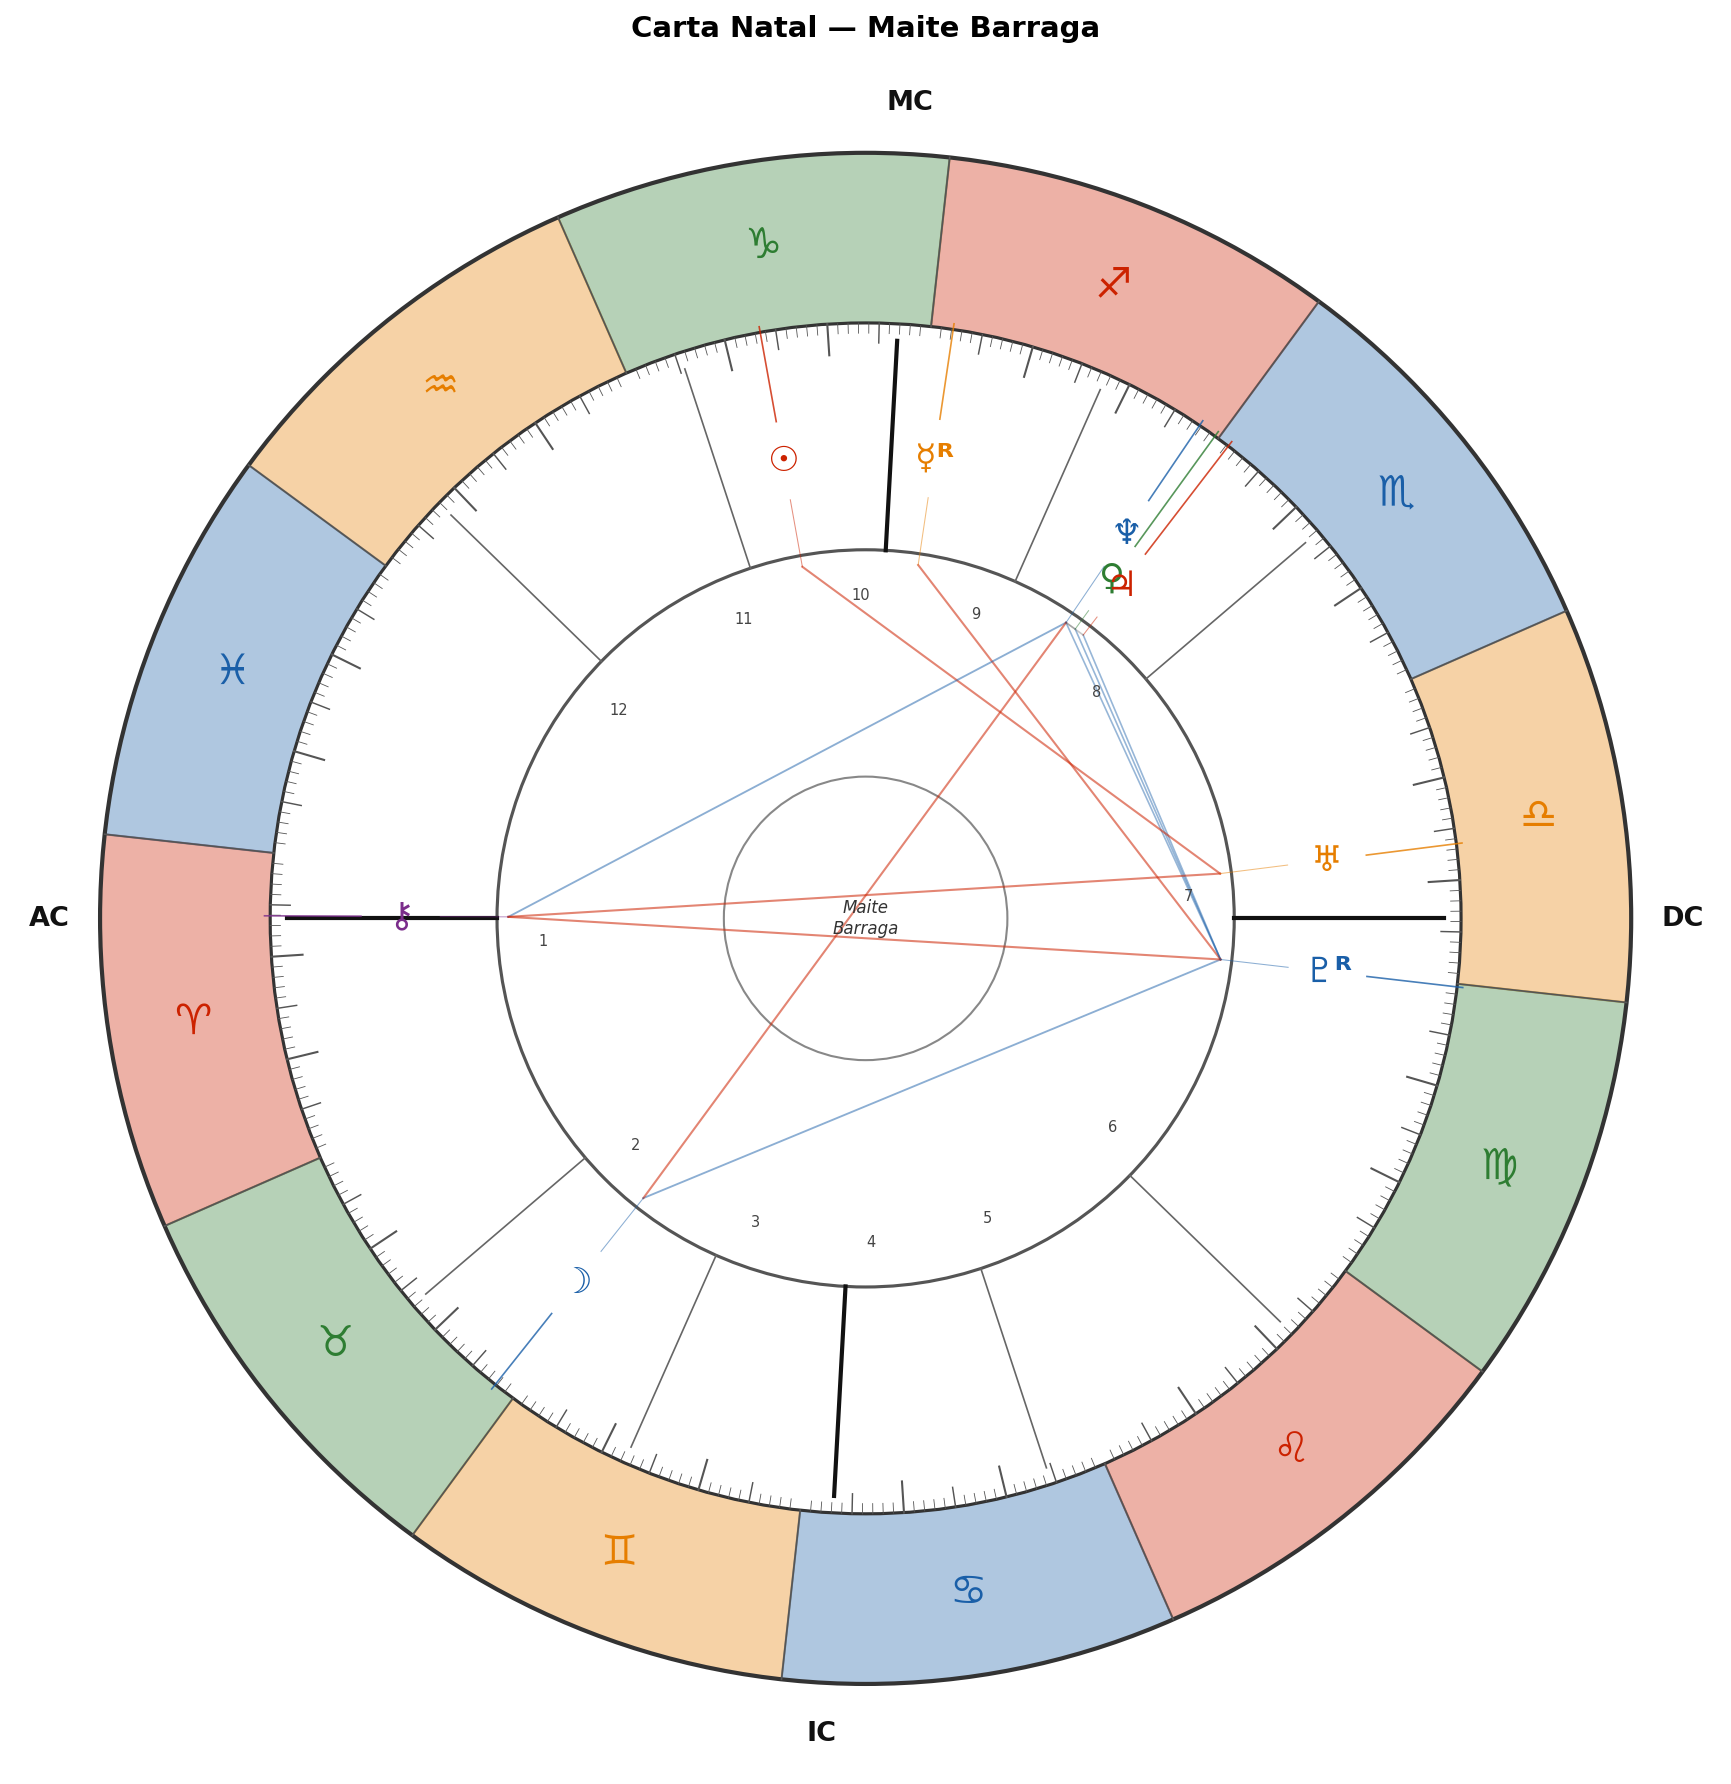
\includegraphics[width=0.72\textwidth]{Maite_Barraga_rueda.png}
\end{center}

\Needspace{3\baselineskip}


% ── Interpretación ────────────────────────────────────────────────────────────
\section{Interpretación — Arquitectura Interna}

\begin{center}
{\small\itshape
No se trata de describir la personalidad. Se trata de mostrar qué procesos\\
de cambio, sensibilidad y transformación pueden activarse en tu vida.
}
\end{center}

\vspace{0.8cm}
\Needspace{5\baselineskip}

% ── 1. Marco general ──────────────────────────────────────────────────────────
\subsection{1. Marco general}

Urano, Neptuno y Plutón no describen lo más cotidiano o visible de tu carta. Muestran procesos más profundos, menos controlables, que pueden modificar tu forma de vivir, sostenerte y atravesar determinadas etapas.

Urano en Libra, Casa 7: muestra dónde aparecen cambios, interrupciones o necesidad de libertad. Cuando se activa, algo que antes funcionaba puede dejar de hacerlo igual.
Neptuno en Sagitario, Casa 8: muestra dónde los límites se vuelven más sensibles, difusos o permeables. Cuando se activa, algo que parecía claro puede perder forma.
Plutón en Virgo, Casa 6: muestra dónde aparecen procesos intensos de transformación. Cuando se activa, algo que se sostenía de una manera ya no puede seguir igual.

Aspectos activos con planetas personales: Urano–Sol en cuadratura (orbe 3.0°), Neptuno–Luna en oposición (orbe 4.35°), Neptuno–Venus en conjunción (orbe 1.8°), Plutón–Luna en trígono (orbe 1.86°), Plutón–Mercurio en cuadratura (orbe 1.85°), Plutón–Venus en sextil (orbe 0.69°).

\vspace{0.8cm}
\Needspace{5\baselineskip}


% ── 2. Urano ──────────────────────────────────────────────────────────────────
\subsection{2. Urano — Ruptura y cambio de patrón}

\subsubsection*{Urano en Libra — Casa 7}

Urano en Libra muestra necesidad de libertad dentro de los vínculos y dificultad para sostener relaciones demasiado rígidas o previsibles. Los cambios suelen aparecer cuando la forma de relacionarte deja de sentirse viva o auténtica.

Puede haber giros importantes en relaciones, acuerdos o maneras de vincularte. A veces necesitas tomar distancia para poder recuperar claridad sobre lo que realmente quieres compartir.

El aprendizaje pasa por construir relaciones donde exista espacio para el cambio sin que cada transformación implique una ruptura.

Urano en Casa 7 muestra necesidad de libertad y autenticidad dentro de los vínculos. Puede costarte sostener relaciones demasiado cerradas, rígidas o previsibles.

A veces aparecen cambios importantes en relaciones, acuerdos o maneras de vincularte. Puede haber necesidad de más espacio o periodos donde revisas profundamente qué significa compartir con otra persona.

El aprendizaje está en construir relaciones donde exista libertad sin que cada cambio implique ruptura.

Urano en cuadratura al Sol genera tensión entre necesidad de estabilidad y necesidad de cambio. Una parte de ti intenta mantener dirección y continuidad, mientras otra necesita romper con lo que ya no encaja.

Puede haber etapas de cambios bruscos, decisiones inesperadas o sensación de no poder sostener durante mucho tiempo la misma orientación.

El aprendizaje pasa por reconocer antes qué necesita actualizarse para no llegar siempre al cambio desde la ruptura.

\vspace{0.8cm}
\Needspace{5\baselineskip}

% ── 3. Neptuno ────────────────────────────────────────────────────────────────
\subsection{3. Neptuno — Disolución y pérdida de forma}

\subsubsection*{Neptuno en Sagitario — Casa 8}

Neptuno en Sagitario puede hacer que busques sentido, dirección o verdad en lugares que después resultan menos sólidos de lo que parecían. A veces necesitas creer en algo para sentir orientación, incluso cuando todavía no está claro.

Puede haber idealización de caminos, proyectos, filosofías o personas que parecen ofrecer amplitud o propósito. También puedes cambiar varias veces de dirección buscando una referencia más auténtica.

El aprendizaje está en desarrollar una visión más consciente sin perder apertura ni capacidad de inspiración.

Neptuno en Casa 8 puede hacer que los procesos emocionales profundos sean difíciles de entender racionalmente. A veces atraviesas cambios internos intensos sin tener todavía palabras claras para explicarlos.

Puede haber mucha sensibilidad hacia lo oculto, lo emocional o lo no visible. También puede costarte distinguir con claridad qué necesitas compartir y qué necesitas proteger.

El aprendizaje está en desarrollar más consciencia emocional sin intentar controlar completamente lo profundo.

Neptuno en oposición a la Luna intensifica la tensión entre necesidad de estabilidad emocional y tendencia a disolver límites internos. A veces sientes mucha conexión emocional con el entorno pero poca claridad sobre tus propias necesidades.

Puede haber confusión emocional, dificultad para sostener estabilidad o tendencia a absorber demasiado de otras personas o ambientes.

El aprendizaje está en desarrollar más diferenciación emocional sin perder sensibilidad.

Neptuno en conjunción con Venus intensifica muchísimo la sensibilidad afectiva y la tendencia a idealizar vínculos o experiencias emocionales. Puede costarte ver con claridad qué ocurre realmente en una relación.

A veces hay mucha entrega, romanticismo o necesidad de conexión profunda, pero también dificultad para sostener límites claros.

El aprendizaje está en amar sin perder completamente la referencia de ti.

\vspace{0.8cm}
\Needspace{5\baselineskip}

% ── 4. Plutón ─────────────────────────────────────────────────────────────────
\subsection{4. Plutón — Intensidad y transformación profunda}

\subsubsection*{Plutón en Virgo — Casa 6 (retrógrado)}

Plutón en Virgo intensifica muchísimo la relación con trabajo, exigencia, control y necesidad de mejora. Puede costarte descansar internamente porque siempre parece haber algo que corregir o perfeccionar.

A veces llevas el esfuerzo y la autoexigencia al límite hasta que el cuerpo o la vida obligan a transformar la manera de funcionar.

El aprendizaje está en desarrollar orden y compromiso sin convertir la exigencia en una forma permanente de presión.

Plutón en Casa 6 intensifica muchísimo la relación con trabajo, hábitos, exigencia y funcionamiento cotidiano. Puede costarte bajar el nivel de control o de presión interna sobre cómo haces las cosas.

A veces llevas el cuerpo, la rutina o la autoexigencia hasta el límite antes de permitir cambios reales en la manera de vivir el día a día.

El aprendizaje pasa por desarrollar formas de organización más sostenibles y menos basadas en tensión constante.

Plutón está retrógrado. La intensidad y la transformación tienden a dirigirse primero hacia dentro. Puede haber procesos profundos que no se ven claramente desde fuera hasta que ya han acumulado mucha fuerza.

Plutón en trígono a la Luna facilita integrar profundidad emocional y capacidad de transformación interna. Las emociones intensas suelen ayudarte a crecer y comprenderte mejor.

Existe capacidad para atravesar procesos emocionales profundos sin perder completamente estabilidad interna.

El aprendizaje pasa por utilizar esa profundidad emocional de forma consciente y constructiva.

Plutón en cuadratura a Mercurio genera tensión entre necesidad de claridad mental y tendencia a intensificar demasiado el pensamiento. A veces la mente entra en procesos muy profundos difíciles de detener.

Puede haber pensamientos repetitivos, dificultad para soltar ideas o tendencia a analizar excesivamente determinadas situaciones.

El aprendizaje pasa por desarrollar más descanso mental sin perder profundidad.

Plutón en sextil a Venus facilita transformar vínculos y patrones afectivos de manera bastante consciente. Existe capacidad para reconocer antes qué relaciones o dinámicas necesitan cambiar.

Las experiencias emocionales profundas suelen ayudarte a comprender mejor qué valoras realmente.

El aprendizaje está en permitir transformación afectiva sin esperar siempre a llegar al límite.

\vspace{0.8cm}
\Needspace{5\baselineskip}

% ── 5. Integración ────────────────────────────────────────────────────────────
\subsection{5. Integración — Las tres fuerzas en tu carta}

Urano, Neptuno y Plutón actúan de formas distintas y no siempre coordinadas. Urano en Libra, Casa 7, muestra dónde aparecen cambios, interrupciones o necesidad de libertad. Cuando se activa, algo que antes funcionaba puede dejar de hacerlo igual. Neptuno en Sagitario, Casa 8, muestra dónde los límites se vuelven más sensibles, difusos o difíciles de sostener. Cuando se activa, algo que parecía claro puede perder forma. Plutón en Virgo, Casa 6, muestra dónde aparecen procesos intensos de transformación. Cuando se activa, algo que sostenías de una manera ya no puede seguir igual.

Neptuno en Sagitario muestra una sensibilidad especial en ciertas áreas de tu vida: tiendes a desbordarte por exceso de impulso o dificultad para frenar a tiempo. Urano en Libra muestra cómo suelen producirse los cambios importantes: los cambios aparecen cuando cambia tu manera de pensar o comprender las cosas. Plutón en Virgo concentra la intensidad en procesos que no pueden quedarse igual indefinidamente: determinadas experiencias terminan empujándote a transformar algo en profundidad.

En determinados momentos, estas tres fuerzas pueden activarse de forma encadenada. Urano en Libra suele aparecer primero: tu manera de pensar o entender una situación cambia bruscamente. Después, Neptuno en Sagitario puede hacer que aparezca sensación de confusión, pérdida de claridad o dificultad para entender bien qué está pasando: la energía pierde dirección y cuesta saber hacia dónde moverte. Finalmente, Plutón en Virgo concentra la intensidad en aquello que ya no puede seguir igual: la presión se concentra en estructuras, recursos o seguridades que necesitan cambiar. Por eso, determinadas etapas pueden sentirse especialmente intensas: no estás viviendo una sola cosa, sino varios procesos moviéndose al mismo tiempo.

\vspace{0.8cm}
\Needspace{5\baselineskip}

% ── 6. Orientación ────────────────────────────────────────────────────────────
\subsection{6. Orientación}

\subsubsection*{Cuando Urano está activo}
Urano suele activarse cuando: cambia bruscamente tu manera de pensar, comprender o comunicar algo. Esto suele sentirse especialmente en temas relacionados con la Casa 7.

\subsubsection*{Cuando Neptuno está activo}
Neptuno suele activarse cuando: pierdes claridad sobre hacia dónde quieres dirigirte. Esto suele sentirse especialmente en temas relacionados con la Casa 8.

\subsubsection*{Cuando Plutón está activo}
Plutón suele activarse cuando: la presión se concentra en estructuras, trabajo, recursos o seguridades importantes. Esto suele sentirse especialmente en temas relacionados con la Casa 6.

\subsubsection*{Cuando no se reconocen}
Cuando estos procesos no se reconocen, es fácil vivirlos únicamente como problemas externos o mala suerte. Sin embargo, muchas veces están mostrando que algo necesita cambiar, redefinirse o transformarse más profundamente.

Intentar sostener exactamente igual algo que internamente ya está cambiando suele generar más desgaste, más confusión o más sensación de bloqueo.

\vspace{0.6cm}
Si estos procesos se ignoran durante mucho tiempo, suelen intensificarse. Urano puede traer cambios cada vez más bruscos. Neptuno puede aumentar la sensación de confusión, desgaste o pérdida de claridad. Plutón puede concentrar tanta intensidad que determinadas situaciones ya no puedan seguir sosteniéndose igual.

Por eso, reconocer antes lo que está cambiando suele ayudar a atravesar estas etapas con más consciencia y menos ruptura.

\vspace{1cm}
\begin{center}
{\small\itshape\color{grisai}
La astrología se usa aquí como lenguaje simbólico de observación, no como definición de la persona.\
Este documento es una aproximación funcional, no un diagnóstico.
}
\end{center}

\end{document}
